\documentclass{beamer}
\mode<presentation>
%\usetheme{PaloAlto}
%\usetheme{Madrid}
\usetheme{AnnArbor}
%\usecolortheme{dolphin}
%\usecolortheme{crane}
\usecolortheme{beaver}
%\usecolortheme{lily}
\setbeamertemplate{background canvas}{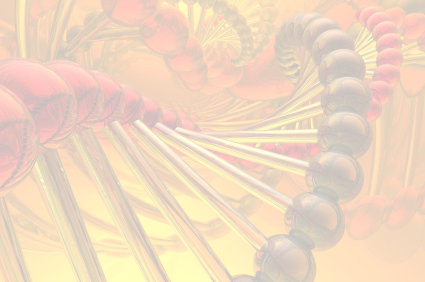
\includegraphics[width=\paperwidth,height=\paperheight]{fotos/fondo.jpg}} 
\usepackage[spanish]{babel}
\usepackage[utf8]{inputenc}
\usepackage{multicol}
\usepackage{xypic}
\title{La variación contínua}
\author{Miguel Burgos \\ \texttt{mburgos@ugr.es}}
\institute[]{Dpto. de Genética e Instituto de Biotecnología \\ CIBM. Lab 127}
\date{Curso 2010-2011}

\setbeamercolor{upcol}{fg=black,bg=yellow}
\setbeamercolor{lowcol}{fg=black,bg=yellow!40}

%\setbeamercolor{upcol}{fg=blue,bg=orange}
%\setbeamercolor{lowcol}{fg=black,bg=blue!20}




\newenvironment{caja}
{
\begin{beamerboxesrounded}[upper=upcol,lower=lowcol,shadow=true]}
{\end{beamerboxesrounded}}

\begin{document}

\begin{frame}
\titlepage
\end{frame}

\begin{frame}
\frametitle{Contenidos}
\tableofcontents[pausesections]
\end{frame}

\section{Caracteres Métricos}

\begin{frame}
\frametitle{Caracteres métricos}
\framesubtitle{Qué son los caracteres métricos}

\begin{caja}{Los caracteres métricos}
\begin{itemize}
\item <1>Diferencias de grado
\item <2->Variación sin discontinuidades naturales=\emph{Variación contínua}
\item <3-4>Caracteres que la exiben = \emph{Caracteres cuantitativos o métricos}
\item <4->La segregación de los genes no puede seguirse individualmente
\item <5>Genética Cuantitativa o Genética Biométrica
\end{itemize}
\end{caja}
\end{frame}

\begin{frame}
\frametitle{Caracteres Métricos}
\framesubtitle{Variación contínua vs. segregación}
\begin{caja}{¿Como la variación discontínua causada por la segregación se traduce en una variación contínua?}
\begin{itemize}[<+-| alert@+>]
\item segregación simultánea de muchos genes
\item Superposición de variación por causas no genéticas
\end{itemize}
\end{caja}

\end{frame}

\begin{frame}
\begin{center}
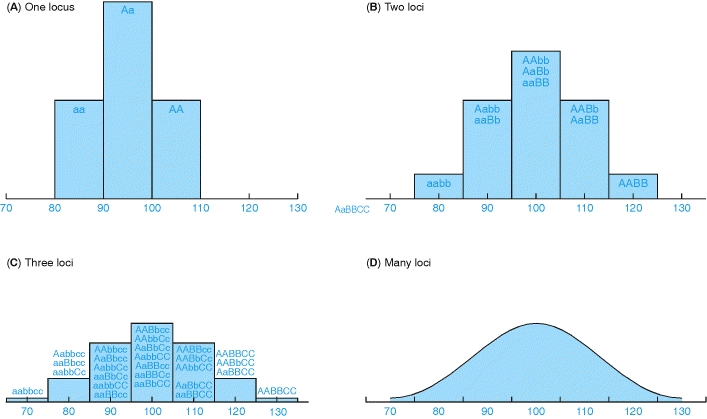
\includegraphics[width=0.8\textwidth]{fotos/ch19f1}
\end{center}
\end{frame}

\begin{frame}
\frametitle{Caracteres Métricos}
\framesubtitle{Variación contínua vs. segregación}
\begin{itemize}[<+-| alert@+>]
\item Genes con efecto grande que causan discontinuidades (genes mayores)
\item Genes con efecto pequeño incapaces de causar discontinuidades (genes menores)
\item La pleiotropía puede hacer que un gen sea clasificado como menor para un carácter y mayor para otro
\item La distinción no es importante y no hay realmente distintas clases de genes
\end{itemize}
\end{frame}

\newtheorem{answeredquestions}[theorem]{Answered Questions}



\begin{frame}
\frametitle{Caracteres Métricos}
\framesubtitle{Variación contínua vs. segregación}
\begin{caja}{Variación poligénica}
Variación causada por la segregación simultánea de muchos genes
\end{caja}
\pause
\begin{caja}{Poligenes}
Genes menores que causan la variación poligénica
\end{caja}
\end{frame}

\begin{frame}
\frametitle{Caracteres métricos}
\framesubtitle{Distribución Normal}
\begin{columns}
\begin{column}{0.4\textwidth}
\begin{caja}{Distribución}
Los caracteres métricos siguen una distribución normal siempre que se elija la escala adecuada
\end{caja}
\end{column}

\begin{column}{0.5\textwidth}
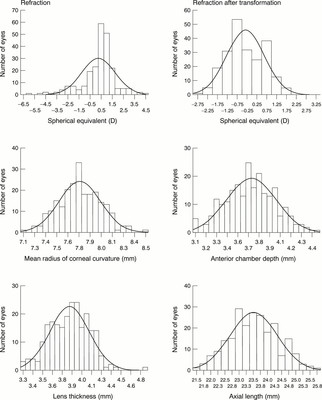
\includegraphics[width=0.9\textwidth]{fotos/distribucion.jpg}
\end{column}
\end{columns}
\end{frame}


\begin{frame}
\frametitle{Caracteres Métricos}
\framesubtitle{Loci de caracteres cuantitativos}
\begin{caja}{¿están realmente los caracteres métricos controlados por muchos loci?}
\begin{itemize}[<+- | alert@+>]
\item Las observaciones concuerdan con lo esperado según la teoría poligénica
\item Evidencia directa con el cartografiado de QTLs
\end{itemize}
\end{caja}
\pause
\begin{caja}{Ejemplo}
\begin{itemize}
\item 17QTL$\rightarrow$quetas esternopleurales. Crom. III \emph{D. melanogaster}
\item 7QTL$\rightarrow$quetas abdominales.
\end{itemize}
\end{caja}
\end{frame}

%**********************************************************

\section{Propiedades de los caracteres métricos}


\begin{frame}
\frametitle{Caracteres Métricos}
\framesubtitle{Propiedades de los caracteres métricos}
\begin{itemize}[<+-| alert@+>]
\item Parecido entre parientes
\item Muchos caracteres estan correlacionados (tamaño $\sim$ nº de crías)
\item Depresión consanguínea $\rightarrow$ disminución del vigor y fecundidad
\item Vigor híbrido o heterosis
\end{itemize}
\end{frame}


\begin{frame}
\frametitle{Caracteres Métricos}
\framesubtitle{Propiedades de los caracteres métricos}
\begin{itemize}[<+-| alert@+>]
\item medias
\item varianzas
\item covarianzas
\item subidivisión en familias $\rightarrow$ componentes de la varianza
\item covarianza entre parientes
\item ....
\end{itemize}
\end{frame}


\section{Efectos genéticos y ambientales}

\begin{frame}
\frametitle{Caracteres Métricos}
\framesubtitle{La suma de efectos genéticos y ambientales}
\begin{caja}{Resumen}
varios o muchos genes intervienen en un carácter$\Rightarrow$existen muchas clases fenotípicas con pequeñas diferencias$\Rightarrow$Variaciones ambientales funden las diferencias entre clases$\Rightarrow$Variación contínua$\Rightarrow$carácter métrico.
\end{caja}
\end{frame}

\end{document}

%diapo simple
\begin{frame}
\frametitle{Caracteres Métricos}
\framesubtitle{Variación contínua vs. segregación}
\end{frame}

%diapo columnas
\begin{frame}
\frametitle{}
\framesubtitle{}
\begin{columns}
\begin{column}{0.5\textwidth}

\end{column}

\begin{column}{0.4\textwidth}

\end{column}
\end{columns}
\end{frame}
